\chapter{Landau Notation}
\label{sec:bigoh}
\index{O-Notation}
\index{Landau Notation}
\index{Asymptotische Abschätzung}
%
Die Informatik ist daran interessiert, Algorithmen (so wie sie im Alltag zur Anwendung kommen) zu optimieren, um Rechenzeit, Speicherplatz und Energie zu sparen. Effizientere Algorithmen erlauben ein wirtschaftlicheres Handeln. Wir benötigen daher ein Werkzeug, um Algorithmen bezüglich ihrer Eigenschaften wie Speicherverbrauch und Laufzeit vergleichen zu können. Obwohl wir nachfolgend von der Laufzeit sprechen, kann die dahinterstehende Theorie genauso auf andere Ressourcen angewandt werden.

Wir bedienen uns einer speziellen mathematischen Notation, welcher die Betrachtung des asymptotischen Verhaltens einer Funktion zugrunde liegt. Diese nennt sich ,,Landau-Notation``, ,,$\mathcal{O}$-Notation``\footnote{In \LaTeX{}  \texttt{\textbackslash mathcal\{O\}} und in Unicode mit U+039F ,,GREEK CAPITAL LETTER OMICRON`` notiert.} oder engl.~``Big O-Notation``. Der Ressourcenverbrauch eines Algorithmus kann durch eine mathematische Funktion beschrieben werden und die $\mathcal{O}$-Notation gibt uns ein relatives Maß, um Algorithmen vergleichen zu können.

Bei den nachfolgenden Beispielen sprechen wir von einer Variable $n$. Es ist jene Variable, die signifikanten Einfluß auf die Effizienz des Algorithmus hat. Bei einem Sortieralgorithmus wird man mit $n$ die Anzahl der Vergleichsoperationen zwischen Elementen beschreiben. Bei der Multiplikation zweier Zahlen wird man die maximale Anzahl der Stellen der beiden Zahlen mit $n$ bezeichnen. Es ist wichtig zu wissen, wofür dieses $n$ konkret steht, doch ergibt es sich aus dem Kontext oft implizit. Im allgemeinen Fall handelt es sich um die Größe der Eingabe.
%
\section{2 grundlegende Klassen}
\subsection{Konstante Laufzeiten}
\index{Konstante Algorithmen}
%
\begin{algorithm}[p]
\caption{Subroutine with constant runtime}
\label{algo:constant}
\lstset{language={python}, label={lst:pyconstant}}
\begin{lstlisting}
def function(n):
    print("Hello World")
    return
\end{lstlisting}
\end{algorithm}
%
Der Algorithmus~\ref{algo:constant} (siehe Seite~\pageref{algo:constant}) nimmt einen Parameter \texttt{n} an und gibt einen leeren Wert zurück. Wir suchen jetzt eine mathematische Funktion, welche uns repräsentiert wieviele Schritte der Algorithmus für eine Eingabe ausführen wird. Für Algorithmus~\ref{algo:constant} gilt: Unabhängig von der Größe von $n$ wird 1 Instruktion ausgeführt\footnote{Die Rückgabe eines Wertes ist stets Teil einer Funktionsverarbeitung und zählen wir daher nicht dazu.}. Wir setzen daher die mathematische Funktion
\[
  f_1(x) = 1
\]
an. Relevant ist hier, dass es sich bei der Zahl $1$ um eine Konstante handelt. Alle Algorithmen deren Effizienz mit einer mathematischen Funktion beschrieben werden können, die nur Konstanten verwendet, fallen in die Klasse ,,konstant``. Also etwa $f_2(x) = 0$ oder $f_3(x) = 365$ als auch $f_1$ haben konstante Laufzeiten. Ganz allgemein: Ein Algorithmus der Ressourcen unabhängig von der Eingabegröße verwendet, besitzt eine konstante Schranke bezüglich dieser Ressource.

Wir haben die Formulierung ,,in eine Klasse fallen`` genutzt. Es bedeutet, dass eine Klasse (wie $\mathcal{O}(1)$) eine Menge von Funktionen ist und unsere gegebene Funktion $f_1$ ist Teil dieser Menge. Alle konstanten Algorithmen sind Elemente von $\On{1}$. Wir schreiben ,,ist Teil von`` mit dem Gleichheitszeichen an\footnote{Das Zeichen $\in$ wird auch genutzt, aber kommt in Fachliteratur selten vor. Wir möchten daher in diesem Dokument der Gleichheitszeichen-Konvention folgen.}:
\[
    f_1 = \On{1} \qquad f_2 = \On{1} \qquad f_3 = \On{1}
\]
%
\subsection{Lineare Laufzeiten}
\index{Lineare Algorithmen}
%
\begin{algorithm}[p]
\caption{Subroutine with linear runtime}
\label{algo:linear}
\lstset{language={python}, label={lst:pylinear}}
\begin{lstlisting}
def function(lst):
    for i in lst:
        print(i)
    return
\end{lstlisting}
\end{algorithm}
%
Der Algorithmus~\ref{algo:linear} benötigt eine lineare Laufzeit. Der Ablauf verrät, dass er über alle Elemente der übergebenen Liste iteriert und damit genau $n$ Schritte benötigt, wenn $n$ die Anzahl der Listenelemente beschreibt. Wird ein $n$ hinzugefügt, benötigt der Algorithmus $1$ Instruktion mehr. Es besteht eine \emph{direkte Proportionalität} zwischen $n$ und der Anzahl von Schritten.

\section{Wozu $\mathcal{O}$ und wie es definiert ist}
%
Angenommen wir hätten zwei Algorithmen. Der erste Algorithmus löst ein gegebenes Problem in konstanter Zeit. Der zweite Algorithmus behandelt das selbe Problem in linearer Zeit. In diesem Fall werden wir den ersten Algorithmus bevorzugen, da dieser Algorithmus bei größeren Eingabedaten trotzdem noch schnell zu einem Ergebnis kommt. Der erste Algorithmus ist ,,effizienter`` (vergleiche mit Tabelle~\ref{tab:constant_vs_linear}).
%
\begin{table}[p]
 \begin{center}
  \begin{tabular}{ccc}
  \hline \hline
   $n$     & Schritte für $f_1$ & Schritte für $f_2$ \\
  \hline
   1       & 1                  & 1 \\
   2       & 1                  & 2 \\
   3       & 1                  & 3 \\
   100     & 1                 & 100 \\
   $10^6$  & 1              & $10^6$ \\
 \hline \hline
  \end{tabular}
  \caption{Zwei Algorithmen, deren Laufzeit mit $f_1(n) = 1$ und $f_2(n) = n$ beschrieben werden können, im Vergleich.}
  \label{tab:constant_vs_linear}
 \end{center}
\end{table}

\index{Obere Schranke}
Wir führen nun die $\mathcal{O}$-Notation ein und untersuchen, ob eine der beiden Funktionen ,,größer`` ist als die andere. ,,Größer`` bedeutet mathematisch wir finden eine Schranke $g(n)$ für eine Funktion $f(n)$, die stets größere Werte liefert als $f(n)$. In diesem Fall sprechen wir von einer ,,oberen Schranke`` und uns interessiert das asymptotische Verhalten.

Wir überlegen uns intuitiv folgende Definition: Eine Funktion $g(n)$ ist die obere Schranke von $f(n)$, wenn\dots
\[
  \forall n \in \mathbb{N}: f(n) \leq g(n)
\]

%Beachte, dass wir hier die Einschränkung treffen, dass wir von positiven Zahlen sprechen. Ein Algorithmus mit negativer Laufzeit ist nur theoretisch vorhanden\footnote{Mit der bisherigen Definition werden wir feststellen, dass $f_2$ keine obere Schranke für $f_1$ bei negativen $n$ darstellt. Wir führen jedoch später ein Konstrukt ein, welches $f_2$ zu einer oberen Schrank macht.} und wird nicht von uns behandelt. \\
Möchten wir $f_4(n) = 1$ und $f_5(n) = n$ vergleichen, können wir $f_4$ als $f(n)$ und $f_5$ als $g(n)$ einsetzen. Wir stellen fest, dass für ein beliebiges, positives $n$ das Ergebnis der Funktion $g(n)$ ein größeres Ergebnis liefert. $f_5$ ist eine obere Schranke von $f_4$.

Wir vergleichen noch zwei andere Funktionen:
\[
   f_6(n) = 42   \hspace{40pt}  f_7(n) = \pi \cdot n
\]
Wir erhalten für $n = 2$ bei $f_6(2) = 42$ und bei $f_7(2) \approx 6,283$. Es ist irgendwie unbefriedigend, dass $f_7$ \emph{keine} obere Schranke von $f_6$ ist, da die Werte von $f_6$ größer als jene von $f_7$ für niedrige $n$ sind. Es ist doch erkennbar, dass ab einem gewissen $n$ die Funktion $f_7$ wesentlich stärker wächst. Daher erweitern wir unsere Definition um einen Mindestwert, ab dem diese Kleiner-Gleich-Relation erst gelten muss.

Wir betrachten eine Funktion (die zB eine Laufzeit beschreibt). Es sei folgende Definition gegeben:
\[
  \On{g(n)} = \{ f(n) \mid \exists n_0 \in \mathbb{N}, \:\forall n \geq n_0: f(n) \leq g(n) \}
\]
Diese Definition erfüllt, was wir erreichen wollen. Wir definieren uns ein sehr großes $n$ für welchen wir den Vergleich der Werte beider Algorithmen (bzw. deren Funktionen) ansetzen und beobachten welche Funktion schneller wächst.

\index{O-Notation!Formale Definition}
Wir treffen jedoch noch eine Entscheidung: Faktoren sind nicht sehr attraktiv. Die Information ,,die Funktion wächst linear`` ist wichtig, aber ob sie mit dem Faktor $2$ oder $3$ wächst, definieren wir als irrelevant. Auch wenn $f_8(n) = 2n$ langsamer wächst als $f_9(n) = 3n$ so sind sie doch sehr ähnlich. Die Entscheidung lässt sich auch mit der Praxis begründen: Moore's Law zeigt uns, dass die Geschwindigkeit von Rechnern exponentiell zunimmt und damit Unterschiede durch Faktoren locker wettmacht. Wir möchten definieren, dass Funktionen mit konstanten Faktoren in der selben Klasse liegen. Wir erweitern unsere Definition ein letztes Mal und führen dazu einen Faktor $c$ ein:
\[
   \On{g(n)} = \{ f(n) \mid \exists c \in \mathbb{R}^+, n_0 \in \mathbb{N},
                  \:\forall n \geq n_0: f(n) \leq c \cdot g(n) \}
\]
%
Diese Definition ist unser formaler Unterbau zur Betrachtung der Landau-Notation.

\section{Kombination von Algorithmen}
%
\begin{algorithm}
\caption{Combination of algorithms}
\label{algo:sequence}
\lstset{language={python}, label={lst:pyseq}}
\begin{lstlisting}
def function(lst):
    for i in lst:
        print(i)
    print("Hello World")
    return
\end{lstlisting}
\end{algorithm}
\begin{algorithm}
\caption{Algorithm with nested algorithms}
\label{algo:nested}
\lstset{language={python}, label={lst:pynested}}
\begin{lstlisting}
def function(lst):
    print("Hello World")
    return

def function2(lst):
    for i in lst:
        function(lst)
        print(i)
    return
\end{lstlisting}
\end{algorithm}
%
Gegeben sei Algorithmus~\ref{algo:sequence}, welcher in zwei Teilbereiche geteilt werden kann. Einerseits haben wir eine Iteration, welche auf eine lineare Laufzeitfunktion in $\On{n}$ hindeutet. Nachfolgend haben wir einen Algorithmus, welcher aus einer Instruktion besteht (konstante Laufzeit in $\On{1}$). Wie verhält sich jetzt die gesamte Laufzeit des Algorithmus? Wir verwenden die Rechenregeln der $\mathcal{O}$-Notation:
%
\[
  f_1(n) = \On{g_1(n)}  \qquad  f_2(n) = \On{g_2(n)}
\] \[
  \Rightarrow f_1(n) + f_2(n) = \On{\max{\left(g_1(n), g_2(n)\right)}}
\] \[
  \Rightarrow f_1(n) \cdot f_2(n) = \On{g_1(n) \cdot g_2(n)}
\]
%
Die erste Regel besagt, dass bei sequentieller Betrachtung der Algorithmen die am stärksten wachsende Funktion die asymptotische Schranke des gesamten Algorithmus angibt. Die zweite Regel beschreibt eine verschachtelte Ausführung wie in Algorithmus~\ref{algo:nested}. Wenn ein Algorithmus einen anderen Algorithmus verwendet, entspricht dies der Multiplikation der Funktionen.

Für Algorithmus~\ref{algo:sequence} berechnen wir:
%
\[
  n + 1 = \On{\max\left(n, 1\right)}
\] \[
  n + 1 = \On{n}
\]
Für Algorithmus~\ref{algo:nested} gilt:
\[
  n \cdot 1 = \On{n \cdot 1}
\] \[
  n \cdot 1 = \On{n}
\]
%
Wir merken uns: Wir müssen immer alle Elemente des Algorithmus betrachten, um die Gesamtlaufzeit angeben zu können.
%
\section{Verallgemeinerung der $\mathcal{O}$-Notation}
\index{O-Notation}
%
Wobei wir hier in unserem Fall von Laufzeiten sprechen, behandelt die Landau-Notation allgemein asymptotisches Verhalten von Funktionen. Wir können für beliebige Ressourcenverwendung eine mathematische Funktion zur Beschreibung heranziehen und durch die $\mathcal{O}$-Notation entsprechende Klassen bilden, um Ressourcenverwendungen zu vergleichen. Liegen zwei Funktionen in der selben Klasse und ein genauer Vergleich ist notwendig, ist eine genaue mathematische Analyse der ignorierten Terme notwendig. Wir haben jedoch vorhin eine Begründung geliefert, dass diese Terme im Allgemeinen nicht relevant sind.

Abseits von der oberen Schranke $\mathcal{O}$ gibt es auch untere Schranken $\Omega$ und exakte Schranken $\Theta$. Um den Umfang dieses Dokuments zu beschränken wird hierauf nicht mehr eingegangen und diese Elemente werden in Lehrveranstaltungen wie \coursedsa{} und \coursedaa{} behandelt.

Weiters möchten wir hier noch folgenden Aspekt diskutieren: Im Algorithmus~\ref{algo:constant} wird von einer Funktion \texttt{print} gesprochen. Doch welche Laufzeit besitzt diese Funktion eigentlich? Über mehrere Abstraktionsebenen hinweg wird es sich letztendlich um eine Sequenz von Maschinenbefehlen handeln. Doch dazu müssten wir die gesamte Maschine analysieren. Wir einigen uns aber in der Theoretischen Informatik darauf, dass die Architektur der Maschine vernachlässigt wird indem stets die Turingmaschine als Referenzmodell herangezogen wird. Die Turingmaschine bietet uns ein universelles Konzept, um Berechenbarkeit erfassbar zu machen. Ein Schritt auf der Turingmaschine ist unsere elementare Einheit. Und unter anderem deshalb ist die Turingmaschine heute genauso wichtig wie zu Zeiten als Rechenmaschinen noch nicht gebaut werden konnten.
%
\index{Obere Schranke}
\begin{figure}[h]
 \begin{center}
  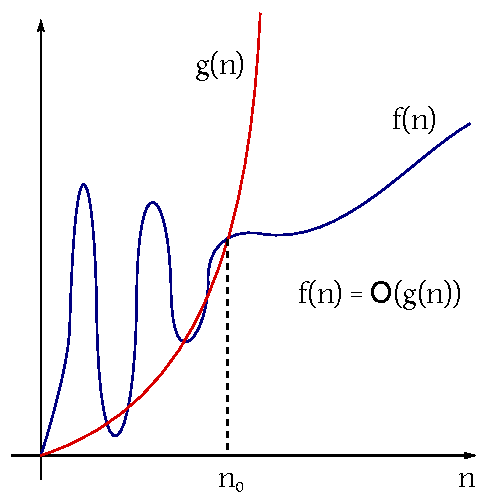
\includegraphics{img/upper_bound.pdf}
  \caption{$g(n)$ bildet eine obere Schranke von $f(n)$}
  \label{fig:upper}
 \end{center}
\end{figure}

\paragraph{Abbildung~\ref{fig:upper}}
Gegeben sei eine beliebige Funktion $f(n)$ mit der oberen Schranke $g(n)$. Wir können ein $n_0$ finden, wobei ab diesem $n_0$ jeder Wert von $g(n)$ größer ist als der Wert von $f(n)$.
%
\section{Weitere Klassen von Funktionen}
%
\subsection{Logarithmische Funktionen}
\index{Logarithmische Algorithmen}
%
Algorithmen mit konstanter Laufzeit werden durch Unabhängigkeit von der Eingabemenge begründet. Die Iteration in proportionaler Abhängigkeit der Eingabemenge definiert die Klasse der Algorithmen mit linearer Laufzeit. Eine weitere Klasse wird durch logarithmisches Verhalten begründet, welche zwischen der konstanten und linearen Klasse einzuordnen ist.

Für Algorithmen mit logarithmischer Laufzeit gibt es ein bekanntes Beispiel. Die Binärsuche ist ein Algorithmus, welcher ein Element in einer geordneten Liste findet. Dazu betrachtet der Algorithmus das mittlere Element der Liste und vergleicht es mit dem gesuchten Wert. Ist es größer, wird die Liste auf die linke Hälfte der Liste reduziert. Ist es kleiner, wird die Liste auf die rechte Hälfte reduziert. Stimmt es überein, haben wir das gesuchte Element gefunden. Dieser Algorithmus setzt sich so lange fort bis das Element gefunden wurde. Die ständige Halbierung der Eingabegröße $n$ beschreibt eine logarithmische Funktion. Daher ist die Binärsuche ein Vertreter der Algorithmen mit logarithmischer Laufzeit.
%
\subsection{Polynomielle Funktionen der Form $n^k$}
\index{Polynomielle Algorithmen}
%
Funktionen der Form $f(n) = n^k$ mit $k \in \mathbb{R}^+$ treten sehr häufig auf. Ein typischer Algorithmus mit solch einer Struktur ist eine verschachtelte Schleife, wobei die Anzahl der Iterationen proportional zu $n$ sein muss. Die Anzahl der Verschachtelungen entspricht $k$.

Liegt in einer Schleife über alle Inputwerte eine Schleife über alle Inputwerte vor, wird pro Wert die gesamte Liste iteriert. Dies entspricht einem Algorithmus dessen Laufzeit mit der Funktion $n^2$ beschrieben werden kann.

Eine offene Frage ist, ob $n^2$ eine andere Klasse als $n^3$ begründet. Da der formale Beweis für den Umfang des Dokuments unangebracht wäre, wird auf diesen verzichtet\footnote{Für formale Beweise ist stets die Ungleichheit der Funktionen in der formalen Definition der $\mathcal{O}$-Notation zu zeigen.} und notiert, dass $n^k$ eine andere Klasse als $n^l$ begründet für beliebige $k$ und $l$ mit $k \neq l$.
\[
  n^3 \notin \On{n^2}
\]
%
\subsection{Exponentielle Funktionen}
\index{Exponentielle Algorithmen}
%
Exponentialfunktionen besitzen eine Struktur $k^n$ mit $k \in \mathbb{R}^+$. Algorithmen, die Untermengen einer Menge mit $n$ Elementen verarbeiten, liegen oft in dieser Klasse, da die Anzahl der Untermengen für eine gegebene Menge $2^n$ ist. Ein anderes Beispiel sind die möglichen Variablenbelegungen für eine boolsche Formel. Sei eine boolsche Formel mit $n$ Variablen gegeben, müssen $2^n$ Variablenbelegungen getestet werden um festzustellen, ob Variablenbelegungen existieren, die diese Formel wahr machen.

Wieder ist es interessant, ob alle Exponentialfunktionen unterschiedlicher Basis in eine Klasse von Funktionen gehören. Auch an dieser Stelle sparen wir uns den formalen Beweis, aber notieren auch hier, dass jede Basis eine eigene Klasse bildet.
\[
  3^n \notin \On{2^n}
\]
%
\section{Die Suche nach der zugehörigen oberen Schranke}
%
Wir sprechen von ,,möglichst großem $n$`` und von ,,Wachstum`` sowie ,,oberen Schranken``. Bei der Angabe von Beispielen zu diesem Thema findet man jedoch die Frage nach der ,,langsamst wachsenden Funktion``. Wie passen diese Dinge zusammen?

Wir haben eine Klasse als Menge von Funktionen definiert. Die Effizienz eines Algorithmus kann durch eine mathematische Funktion beschrieben werden. Daher wissen wir in welcher Klasse ein Algorithmus liegt. Weiters bilden diese Mengen Untermengen von anderen Klassen. Wir sprechen hier von ,,oberen Schranken``, die nach unten hin offen sind. Ein Algorithmus mit linearem Laufzeitverhalten ist gleich effizient wie ein anderer linearer Algorithmus und effizienter als konstante oder logarithmische Algorithmen. Es bildet sich also eine Hierarchie:

\[
  A \rightarrow B \qquad \text{,,B ist effizienter als A``}
\] \[
  \text{konstant} \rightarrow
  \text{logarithmisch} \rightarrow
  \text{linear} \rightarrow
  \vspace{-8pt}
\] \[
  \text{polynomiell mit $n^k$} \rightarrow
  \text{exponentiell mit $k^n$}
\] \[
  k \in \mathbb{R}^+, n \in \mathbb{N}
\]

Es können noch weitere Klassen definiert werden, um Algorithmen noch besser zu klassifizieren. Allerdings handelt es sich bei diesen Klassen um einen guten Überblick. Wir notieren weiters, dass alle Klassen kleiner oder gleich ,,polynomiell mit $n^k$`` durch einen Polynom\footnote{Mathematische Struktur der Form $y_0x^0 + y_1x^1 + y_2x^2 + \ldots + y_nx^n$.} beschrieben werden können und daher mit ,,Algorithmen polynomieller Laufzeit`` bezeichnet werden. Es ist gängige Konvention polynomielle Algorithmen als ,,effizient`` zu bezeichnen und andere (insbesondere exponentielle Algorithmen) als ,,ineffizient``.

Wir könnten nun alle Funktionen mit $\On{n^n}$ abschätzen und stellen fest, dass diese Klasse alle praxisrelevanten Algorithmen umfasst. Allerdings würde es uns nicht weiterhelfen die Effizienz eines Algorithmus zu erfassen. Wir suchen daher für einen Algorithmus jene mathematische Funktion, die den Algorithmus möglichst genau beschreibt. Wir wählen keine zu große Schranke, um gute Klassifikation zu erreichen. Wir wählen keine zu kleine Funktion, da dies keine obere Schranke der Funktion wäre. Mit ,,langsamst wachsende Funktion`` ist also die kleinstmögliche (aber formal korrekte) ,,obere Schranke`` gemeint.
%
\section{Zusammenfassung}
\index{O-Notation!Intuitive Erklärung}
%
In den vorigen Kapiteln haben wir uns einige Formalismen mit Hinweis auf andere Lehrveranstaltungen erspart. Zugleich haben wir kein intuitives Verständnis der $\mathcal{O}$-Notation entwickelt. Zweiteres wollen wir in diesem Abschnitt nachholen.

Gegeben sei ein Algorithmus. Wir untersuchen wie stark die Laufzeit des Algorithmus von der Eingabe abhängt. Auf Basis dieser Information bilden wir eine mathematische Funktion, die dieses Verhalten beschreibt. Wir reduzieren dann die Funktion auf eine Repräsentation, welche für die jeweilige Klasse repräsentativ ist. Dies können wir mit folgenden Regeln durchführen (beachte dass dieses Modell nicht vollständig ist, aber für die Betrachtung einfacher Polynome ausreicht):
%
\begin{enumerate}
  \item Sind zwei Funktionen durch eine Addition verbunden (Exponenten dürfen nicht als eigenständige Funktion betrachtet werden), reduzieren wir die Funktion auf jenen Summanden, der die größte obere Schranke besitzt.
  \item Eine Funktion der Struktur $an^{b}$ (mit $a$ und $b$ als Konstanten) reduzieren wir auf $n^b$.
  \item Eine Funktion der Struktur $ab^{cn + d}$ (mit $a$, $b$, $c$ und $d$ als Konstanten) reduzieren wir auf $e^n$ mit $e=b^c$. Dem liegt die Rechenregel $n^{km} = {(n^k)}^m$ zugrunde.
\end{enumerate}

Wir möchten ein paar Beispiele durchgehen. Die Funktion $f(n) = 3n^2 + n$ können wir zuerst mit Regel (1) bearbeiten. Wir sehen, dass die Funktion aus einer quadratischen Teilfunktion $3n^2$ und einer linearen Funktion $n$ besteht. Wir wissen aufgrund der Klassifikationen, dass die quadratische Funktion schnell wächst. Daher möchten wir die Funktion auf $f(n) = 3n^2$ reduzieren. Nun wird unsere Struktur durch Regel (2) beschrieben und wir ersetzen sie dementsprechend mit $n^2$. Das heißt unsere finale Klasse in der $f$ liegt, nennt sich $\mathcal{O}(n^2)$.

Für das Beispiel $f(n) = 5^n + n^2 - 5$ gilt: $5^n + n^2 - 5 \stackrel{(1)}{\Rightarrow} 5^n  \Rightarrow \mathcal{O}(5^n)$. In Tabelle~\ref{tab:classes} wird nochmals ausgeführt welche Relationen zwischen den Klassen besteht.

\index{O-Notation!Beispiele}
Ich möchte allerdings auch nicht verneinen, dass wir Themen offen gelassen haben. Ich möchte wieder auf weiterführende Lehrveranstaltungen verweisen, aber trotzdem einen Überblick geben:
\begin{itemize}
  \item Was ist wenn wir eine beschränkte Problemgröße haben? $n$ kann nicht ins Unendliche wachsen. In diesem Fall eignet sich die $\mathcal{O}$-Notation nicht gut.
  \item Kann ich mehrere Input-Variablen modellieren?
  \item Wie analysiert man rekursive Funktionen?
  \item Wie stehen obere, untere und exakte Schranken zueinander? Welche Rechenregeln ergeben sich?
\end{itemize}
%
\begin{table}[ht]
 \begin{center}
  \begin{tabular}{cl}
   Klasse & Beschreibung \\
  \hline
   $\On{1}$ & konstant \\
   $\On{\log{n}}$ & logarithmisch \\
   $\On{n}$ & linear \\
   $\On{n^2}$ & quadratisch \\
   $\On{n^3}$ & kubisch \\
   $\On{n^k}$ & polynomiell $k$-ten Grades (mit $k>3$) \\
   $\On{2^n}$ & exponentiell zur Basis 2 \\
   $\On{3^n}$ & exponentiell zur Basis 3 \\
   $\On{k^n}$ & exponentiell zur Basis $k$ \\
%   $\On{n!}$ & faktoriell \\
  \end{tabular}
  \caption{Klassen nach $\mathcal{O}$-Notation}
  \label{tab:classes}
 \end{center}
\end{table}

Beispielfunktionen und deren Klassenzugehörigkeit sind in Tabelle~\ref{tab:function_cheatsheet} gegeben.
\begin{table}[p]
 \[
   f_1(n) = 1 \mathspace
   f_2(n) = 42 \mathspace
   f_3(n) = \log{n} \mathspace
   f_4(n) = \log_2{n} \mathspace
 \] \[
   f_5(n) = n \mathspace
   f_6(n) = 2n \mathspace
   f_7(n) = n^2 \mathspace
 \] \[
   f_8(n) = n^3 \mathspace
   f_9(n) = 3^n \mathspace
   f_{10}(n) = 3^{n+1}
 \]
 \vspace{20pt}
 \begin{center}
  \begin{tabular}{cccccccc}
  \hline \hline
   $=$      & $\On{1}$   & $\On{\log{n}}$ & $\On{n}$   & $\On{n^2}$ & $\On{n^3}$ & $\On{2^n}$ & $\On{3^n}$ \\
  \hline
   $f_1$    & \checkmark & \checkmark     & \checkmark & \checkmark & \checkmark & \checkmark & \checkmark \\
   $f_2$    & \checkmark & \checkmark     & \checkmark & \checkmark & \checkmark & \checkmark & \checkmark \\
   $f_3$    & \xmark     & \checkmark     & \checkmark & \checkmark & \checkmark & \checkmark & \checkmark \\
   $f_4$    & \xmark     & \checkmark     & \checkmark & \checkmark & \checkmark & \checkmark & \checkmark \\
   $f_5$    & \xmark     & \xmark         & \checkmark & \checkmark & \checkmark & \checkmark & \checkmark \\
   $f_6$    & \xmark     & \xmark         & \checkmark & \checkmark & \checkmark & \checkmark & \checkmark \\
   $f_7$    & \xmark     & \xmark         & \xmark     & \checkmark & \checkmark & \checkmark & \checkmark \\
   $f_8$    & \xmark     & \xmark         & \xmark     & \xmark     & \checkmark & \checkmark & \checkmark \\
   $f_9$    & \xmark     & \xmark         & \xmark     & \xmark     & \xmark     & \xmark     & \checkmark \\
   $f_{10}$ & \xmark     & \xmark         & \xmark     & \xmark     & \xmark     & \xmark     & \checkmark \\
 \hline \hline
  \end{tabular}
  \caption{Klassifikation der Funktionen $f_1$ bis $f_{10}$. Wähle eine Funktion (Zeile) und schaue nach ob sie in der Klasse (Spalte) enthalten ist. $\checkmark$ für ,,Ja`` und \xmark{} für ,,Nein``.}
  \label{tab:function_cheatsheet}
 \end{center}
\end{table}
